\section{Data separability} \label{sec:dataSeparability}
Besides evaluating the user performance in real-time, it would be beneficial to evaluate the clustering of feature values used to fit the classifier and regressors off-line. This will provide information on how the clusters between classes separates and how the feature values within clusters bundle. %Thus it can be evaluated between sessions if the clusters are more distinguished and thereby easier for the classifier and regressors to discriminate between. 
By doing this between sessions it can be evaluated how distinguishable the clusters are to judge how well the classifier and regressors will discriminate between the different clusters. For this purpose a Principle Component Analysis (PCA) will be utilized to reduce the dimensionality of the feature space, from which is subsequently can be used to calculate the distance between clusters and distances from feature values to centroids within clusters. The following section provides theoretical information on the PCA procedure. 


\subsection{Principal Component Analysis} \label{sub:PCA}
PCA is used to express a set of possibly correlated variables into uncorrelated components, called principal components (PC). A dataset of many variables can thus be expressed in a reduced dimensionality hyperspace using less variables that are the most defining for the given dataset. Each principal component is orthogonal on the former and are uncorrelated and have zero covariance. They each define the largest variance in an axis, such that the first PC describes the direction of the maximum variance of the dataset. Each following PC describes the next highest variance of the dataset, with the constraint that it is orthogonal and has zero covariance with any of the former PCs. \cite{Semmlow2014}
PCA is the orthogonal projection of data onto a lower dimension linear space. A PC is found by minimizing the variance by projecting the feature values, the red dots in \figref{projection}, onto the line describing the highest variance in the data set (purple line) as seen on \figref{projection}. The PC (purple line) is found by minimizing the mean square distance between the data points. \cite{Semmlow2014}

\begin{figure}[H] 
	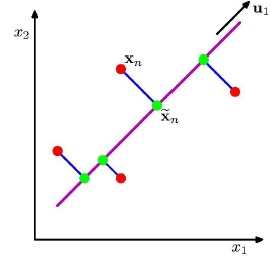
\includegraphics[width=0.3\textwidth]{figures/zASP/projection}
	\caption{Projection of feature values (red dots) onto PC axes (purple).}
	\label{projection}
\end{figure}
\vspace{-10pt}
The algebraic method of calculating the PCs can be done by using Singular Value Decomposition (SVD). The first step is to compute the squared cross product matrix of variances and covariances among every pair of the variables in the data set, where the diagonals are the variances and the off-diagonals are the covariances, as done in the following equation \cite{Semmlow2014}:
%\vspace{-20pt}
\begin{equation}
S = X \textquoteright X
\end{equation}
Where S is the cross product and X is the feature set matrix. When finding the PCs it includes an eigen-analysis of S. The eigenvalues of are solutions to the following equation \cite{Semmlow2014}:
%\verticalspace{1}
\begin{equation}
| S - \lambda I |  = 0
\end{equation}
Where $\lambda$ is the variance of each PC and $I$ is the identity matrix. After solving for $\lambda$ the eigenvectors can be solved through the following equation \cite{Semmlow2014}:
\begin{equation}
det | S - \lambda I | b_{i} = 0
\end{equation}
Where $b_{i}$ is used to calculate the eigenvectors as in \cite{Semmlow2014}:
\begin{eqnarray}
u_{i} = \frac{b_{i}}{\sqrt{b_{i}^{\textquoteright} b_{i}}}
\end{eqnarray}
Where $u_{i}$ is the $i^{th}$ number of eigenvectors. The number eigenvectors equal the dimension size of the original feature space. 
The SVD orders the eigenvalues by size, so that $\lambda_{1} > \lambda_{2} … > \lambda_{i}$. The scores for each PC is equal to the corresponding eigenvalue for that exact axis. The eigenvalues describe how much of the variance is accounted for by the associated PC. Summation of all eigenvalues accounts for the total variance of the data set; this is called the trace. To find how much the each PC accounts for, the eigenvalue of that PC is divided by the total variance: $\%~ of~ total~ variance~ = \frac{\lambda_{i}}{Trace}$. Deciding how many PCs the feature space should be reduced to, by setting a threshold of how much of the total variance should be preserved. \cite{Semmlow2014}

\subsection{Distance measure} \label{sub:distanceMeasure}
After reducing the dimensionality of the original feature set the clusters can be analysed. For the purpose of measuring distances between and within clusters the centroid of each cluster must be calculated, as in \eqref{eq:centroid}:

\begin{equation} \label{eq:centroid}
	C = \Bigg[ \frac{[x_1+x_2 +~...~+ x_i],[y_1+y_2 +~...~+ y_i] ,~...~,[k_1+k_2 +~...~k_i]}{k} \Bigg]
\end{equation}

Where $C$ is the centroid, $i$ is the number of feature point in a dimension and $k$ is the number of dimensions. To calculate the distance between centroids of clusters the Euclidean distance (ED) is computed. The ED is the length of the a line segment connecting points, in this case in form of two centroids $p$ and $q$. The calculation of ED in a $k$-dimensional space is as in \eqref{eq:euclidiandistance}:

\begin{equation} \label{eq:euclidiandistance}
	ED(p,q) = \sqrt{(p_1-q_1)^2 + (p_2-q_2)^2~+~...~+ (p_k-q_k)^2}
\end{equation} 

When calculating the distance from feature values in a cluster to their corresponding centroid the ED is computed likewise. To get a general impression of the distance from the feature values constituting the cluster to the centroid of the cluster the average of the distances is calculated. 

from feature values of a cluster to their centroid, the average distance from all feature values to their centroid is calculated. 




